\documentclass[smaller,a4paper,allowframebreaks]{beamer}
\usepackage{amsmath,amssymb,pdfsync,listings}
\usepackage{verbatim}
\usepackage{graphicx}
\usepackage{truncate}
\usepackage[final]{pdfpages}
\usepackage{times}
\usepackage{pgffor}
\usepackage{listings}
\usepackage[english]{babel}

\begin{document}
\title{Exceptions}
\frame{\titlepage}

\begin{frame}
\frametitle{Excercise 1 : Cholesky Decomposition}
\begin{itemize}
\item Implement a safe decomposition method for full matrices
      \begin{itemize}
            \item Store the matrix column-wise in a std::vector<double>             
            \item Attempt Cholesky decomposition
            \item If decomposition fails raise an exception
            \item Catch the exception and fall bacck to LU with pivoting
            \item A reference implementation of LU is provided in Matlab language
            \item Alternatively use the matrix class from excercise 3 and extend it adding a cholesky method
            \item For Cholesky use the following formulas :\\[3mm]
            \center{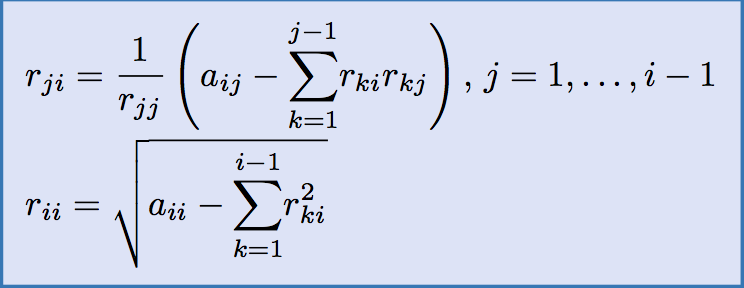
\includegraphics[width=.75\linewidth]{chol.png}}
      \end{itemize}      
\end{itemize}
\end{frame}


\begin{frame}
\frametitle{Exercise 2 : Robust Newton Iteration}
\begin{itemize}
\item Implement a more robust version of the Newton solver
      \begin{itemize}
            \item Read the function from the command line and validate input
            \item Try a Newton step, if the residual is not decreased use a damping parameter
            \item If the damping parameter becomes too small switch to bisection
      \end{itemize}      
\end{itemize}

\end{frame}

\end{document}


